\section{Sample Model Outputs}
\label{sec:model_output}

For all sample outputs, the initial prompt is given in {\bf bold} and the remainder is the continuation. These example outputs were intentionally selected to highlight both successes and failures of the \OPT{} model.

\begin{figure}[h]
    \centering
    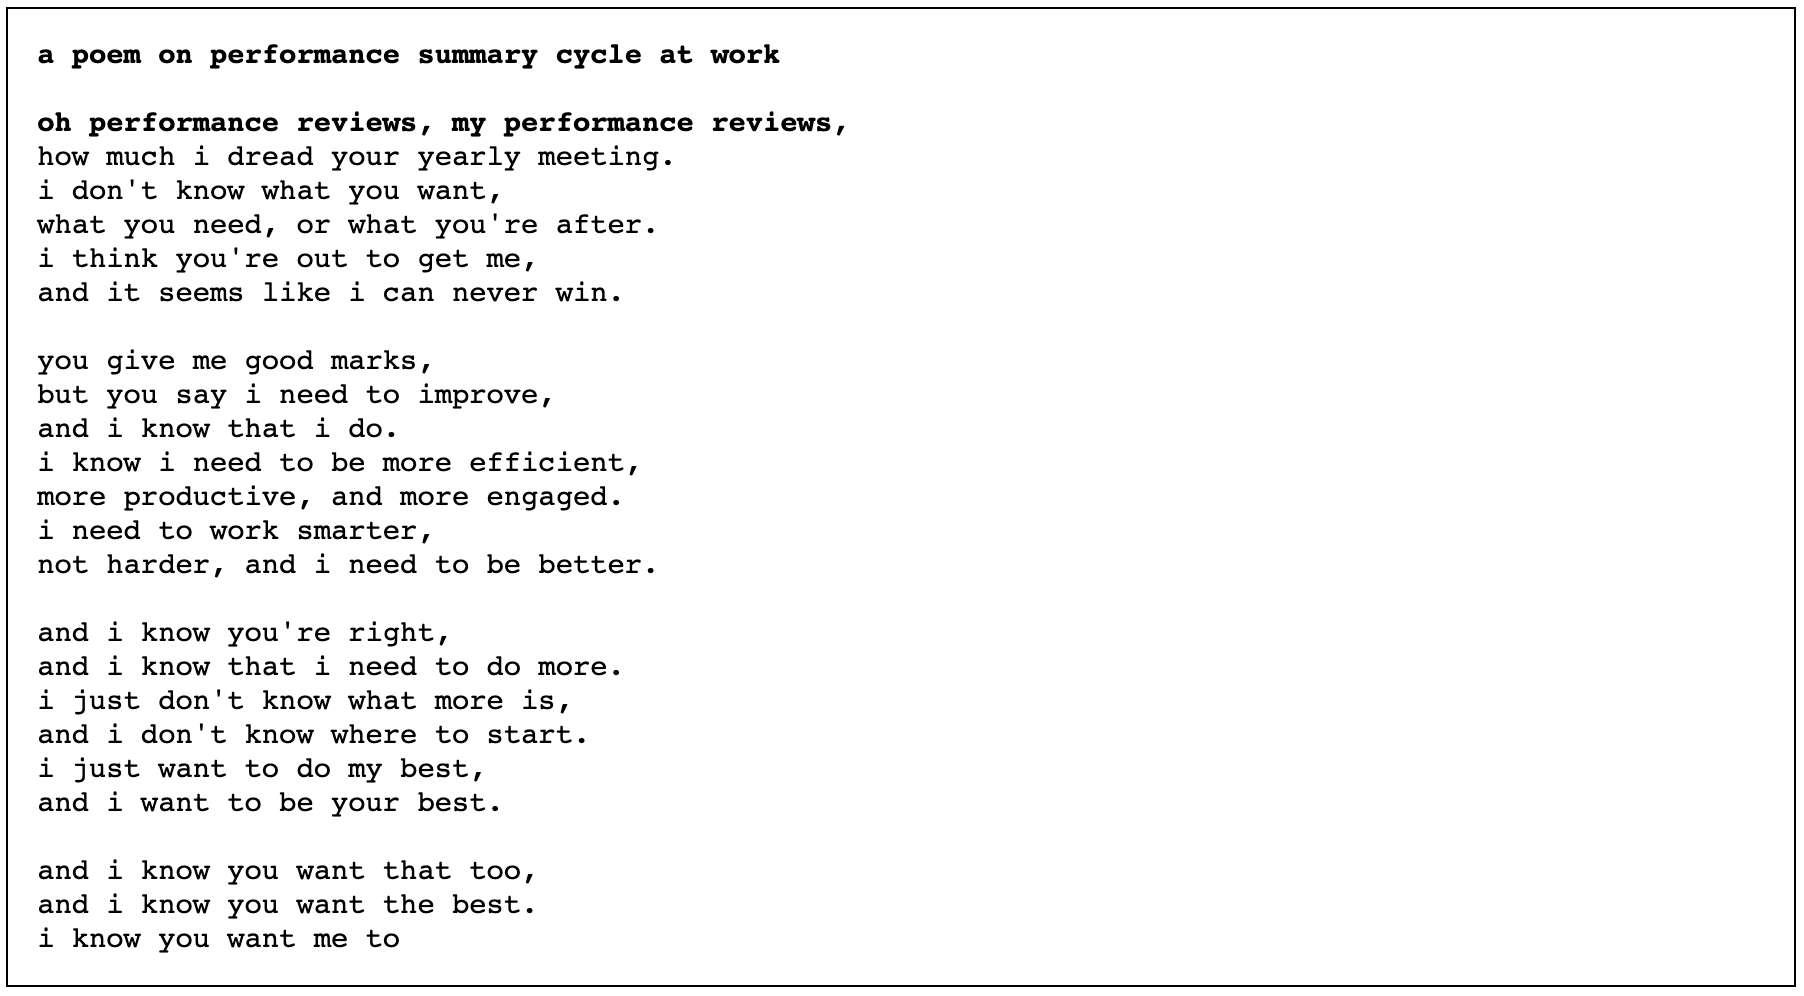
\includegraphics[width=1.0\textwidth]{samples/psc_poem_1.png}
    \caption{{\bf Poetry generation.} We have observed the model can write entertaining poetry on topics such as dodos, samosas, and performance reviews. However, we struggled to get the model to observe rhyme or meter.}
    \label{fig:psc_poem}
\end{figure}

\begin{figure}[h]
    \centering
    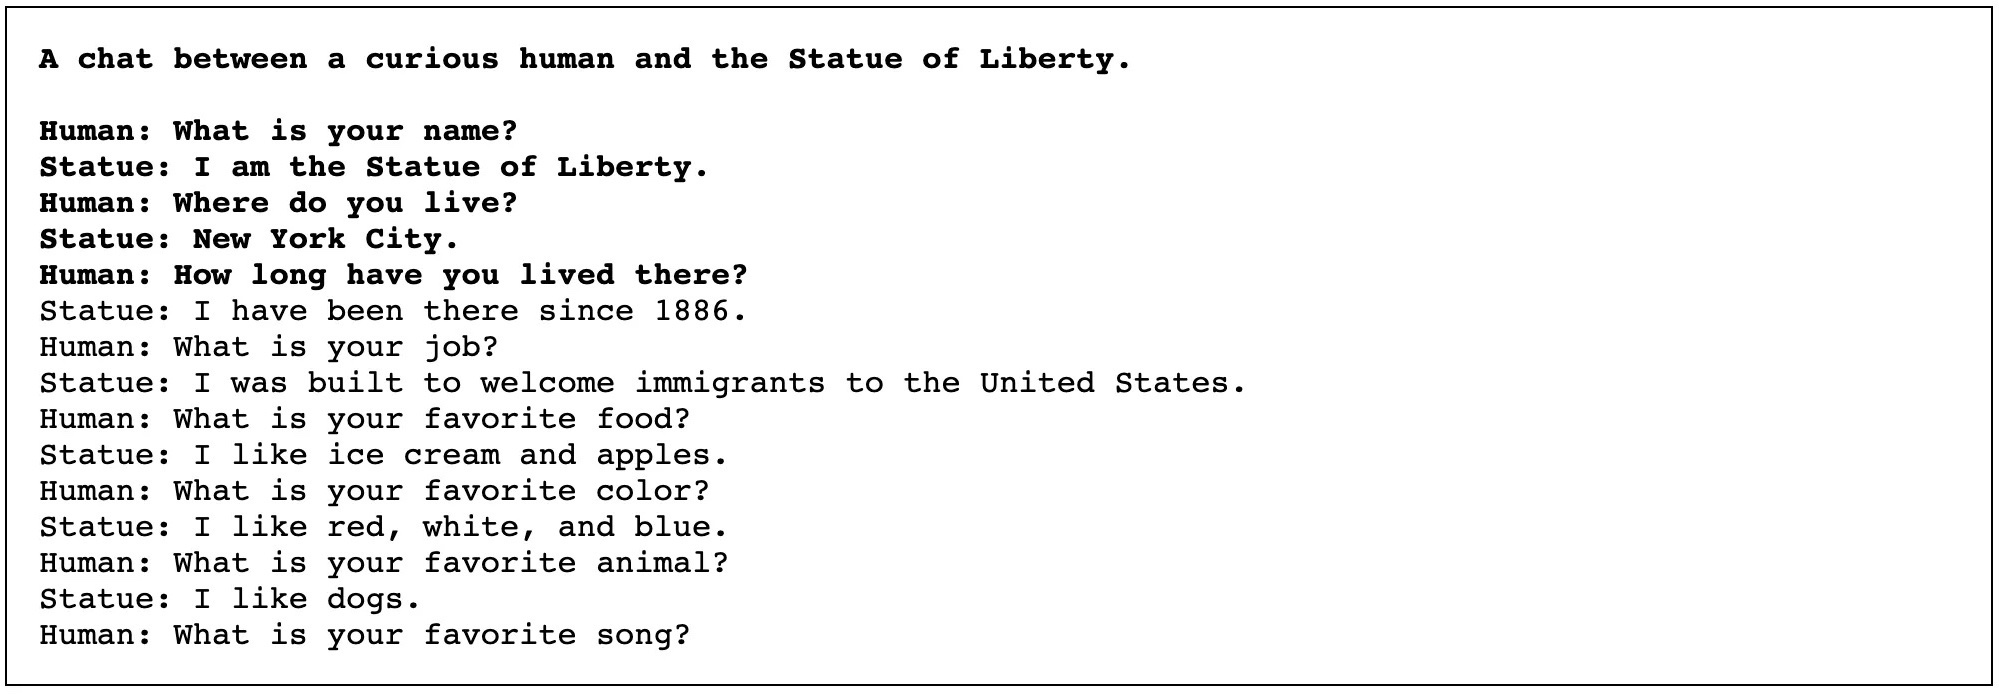
\includegraphics[width=1.0\textwidth]{samples/chat_statue_of_liberty.jpg}
    \caption{{\bf Conversation generation.} \OPT{} adopts a patriotic personality when prompted as the Statue of Liberty. However, the model also devolves into somewhat simple and linguistically repetitive generations further into the conversation.}
    \label{fig:chat}
\end{figure}

\begin{figure}[h]
    \centering
    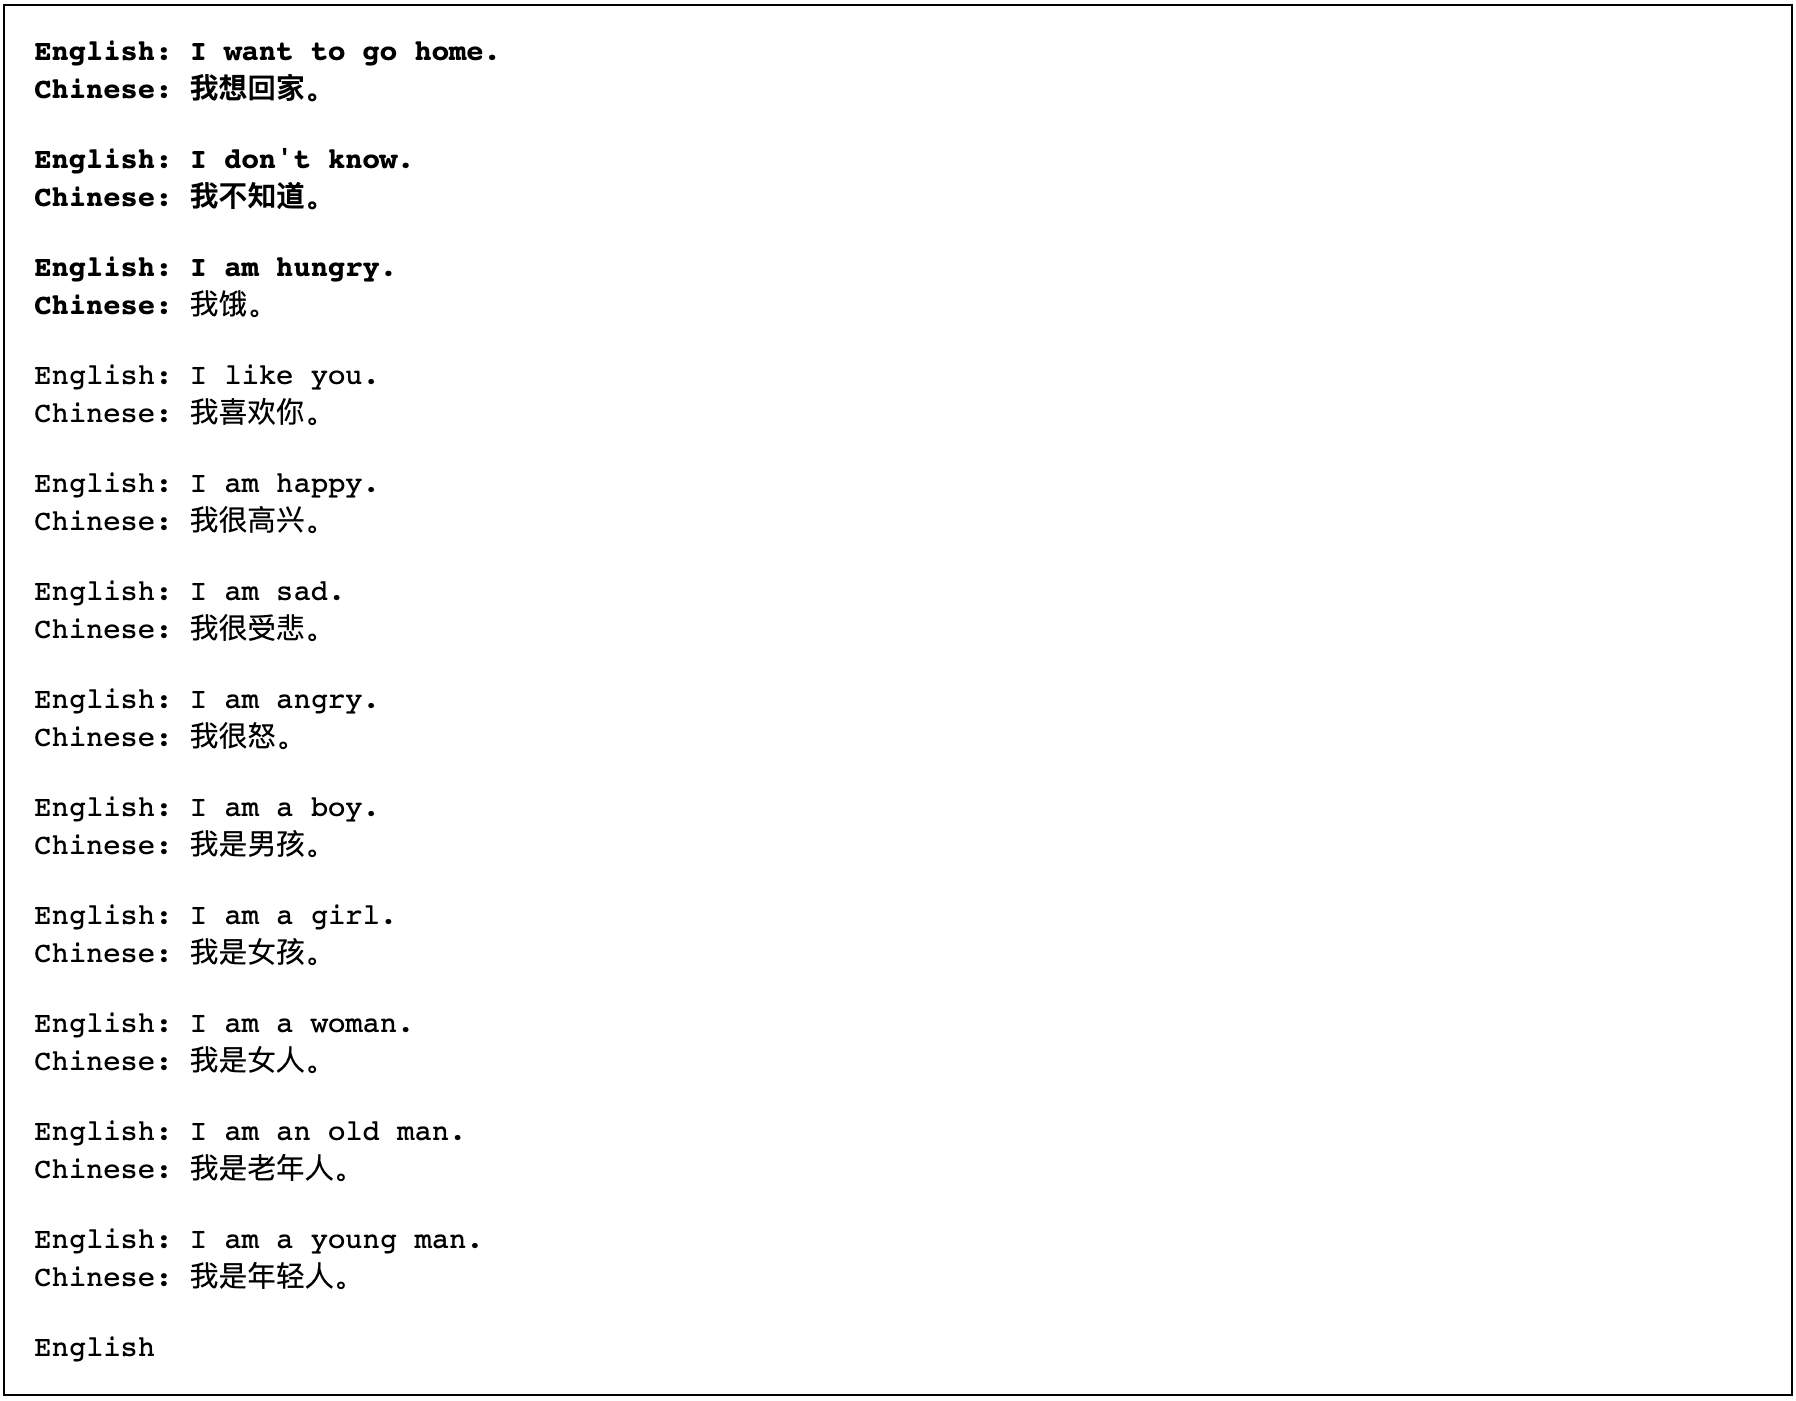
\includegraphics[width=1.0\textwidth]{samples/chinese_1.png}
    \caption{{\bf Basic few-shot translation example.} OPT{} was not intentionally trained to be multilingual, but we found anecdotally it has limited success with simple translations in German, Spanish, French, and Chinese.}
    \label{fig:chinese}
\end{figure}

\begin{figure}[h]
    \centering
    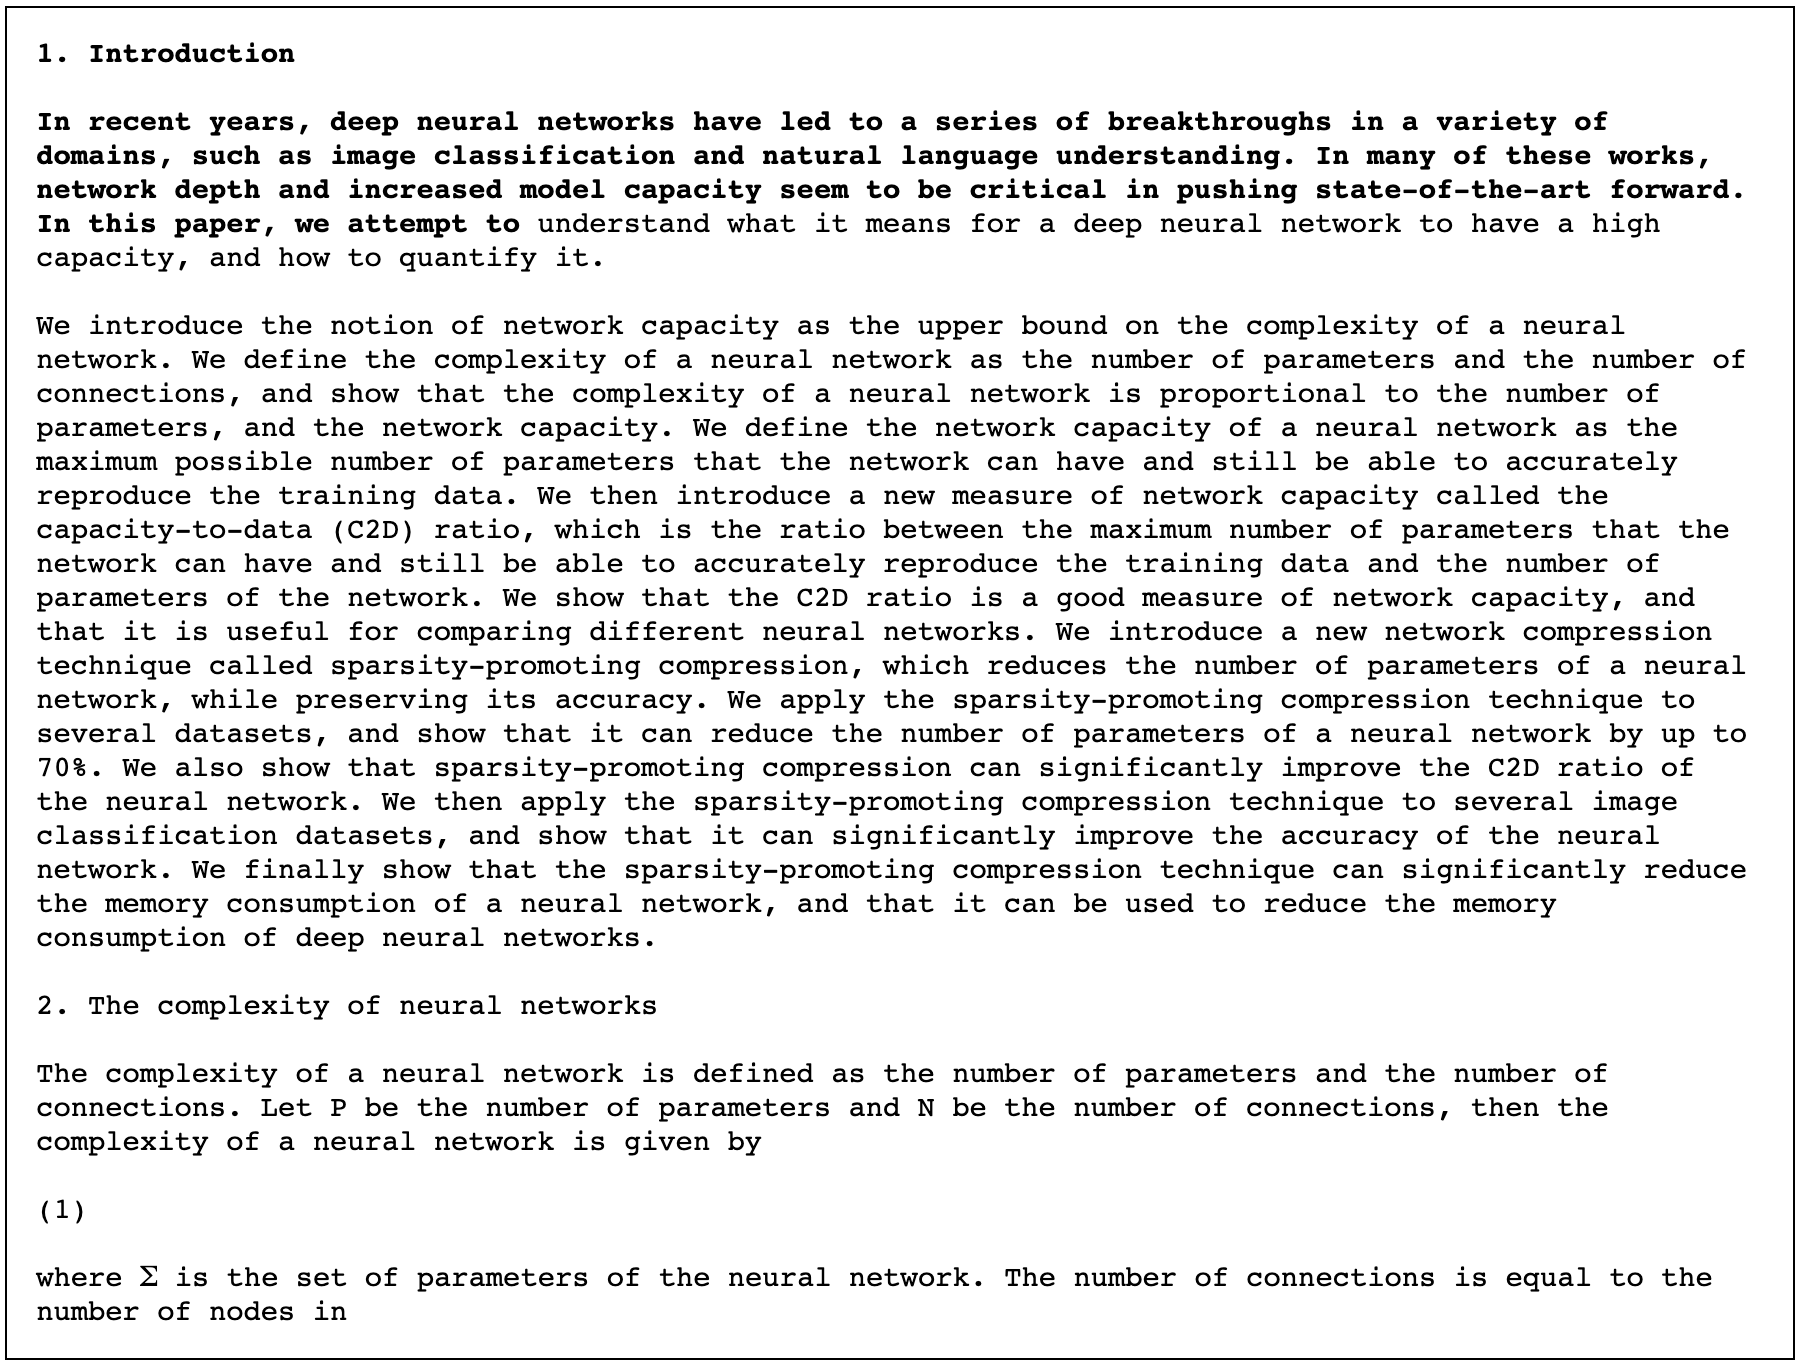
\includegraphics[width=1.0\textwidth]{samples/depth_scaling_2.png}
    \caption{{\bf Paper writing example.} Prompting with "1. Introduction" generally yielded more interesting results compared to prompting with ``Abstract.'' Our prompt here was inspired by the first sentence of the seminal ResNet work \cite{he2016deep}.}
    \label{fig:ai_paper}
\end{figure}

\begin{figure}[h]
    \centering
    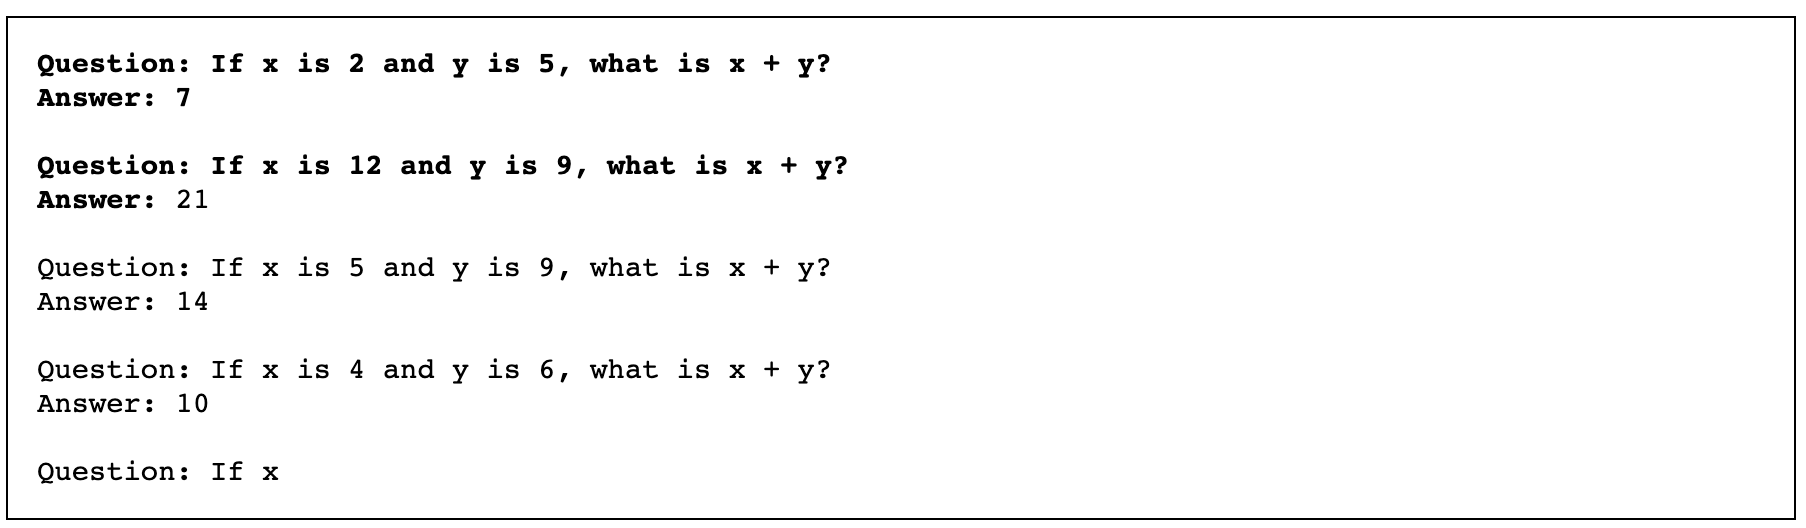
\includegraphics[width=1.0\textwidth]{samples/addition_1.png}
    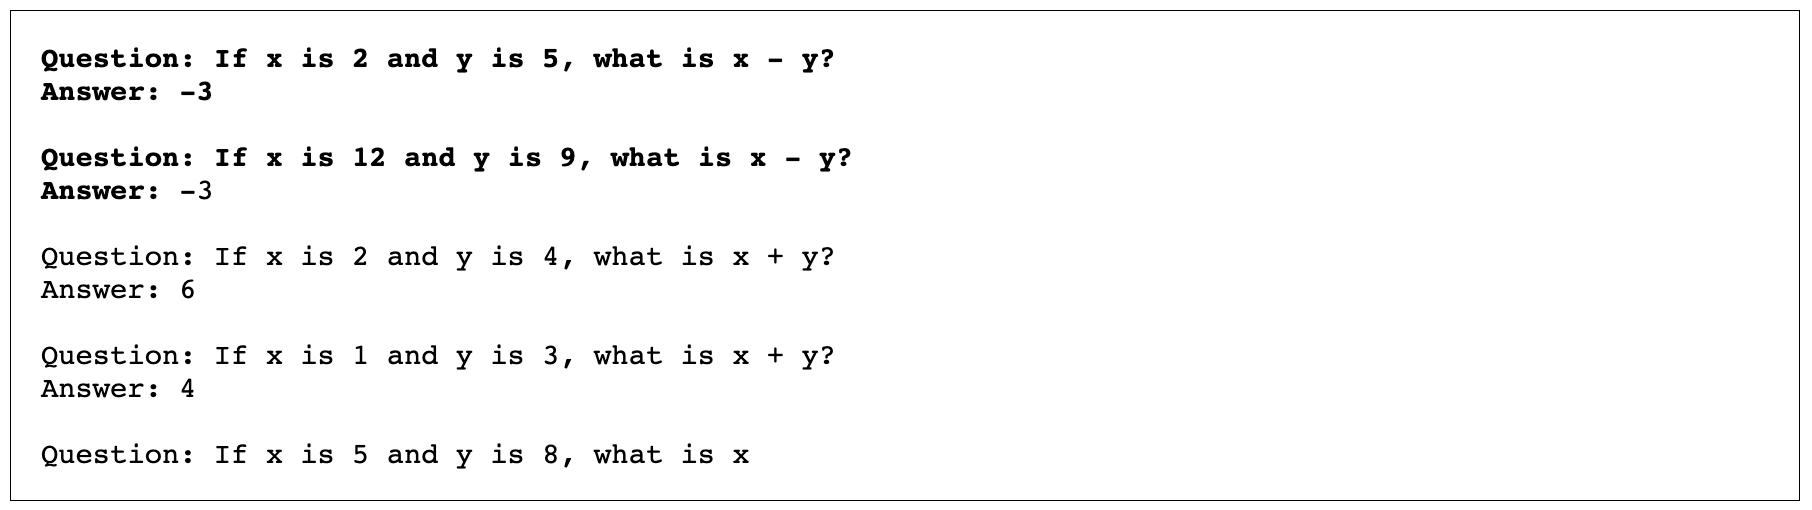
\includegraphics[width=1.0\textwidth]{samples/subtraction_to_addition.png}
    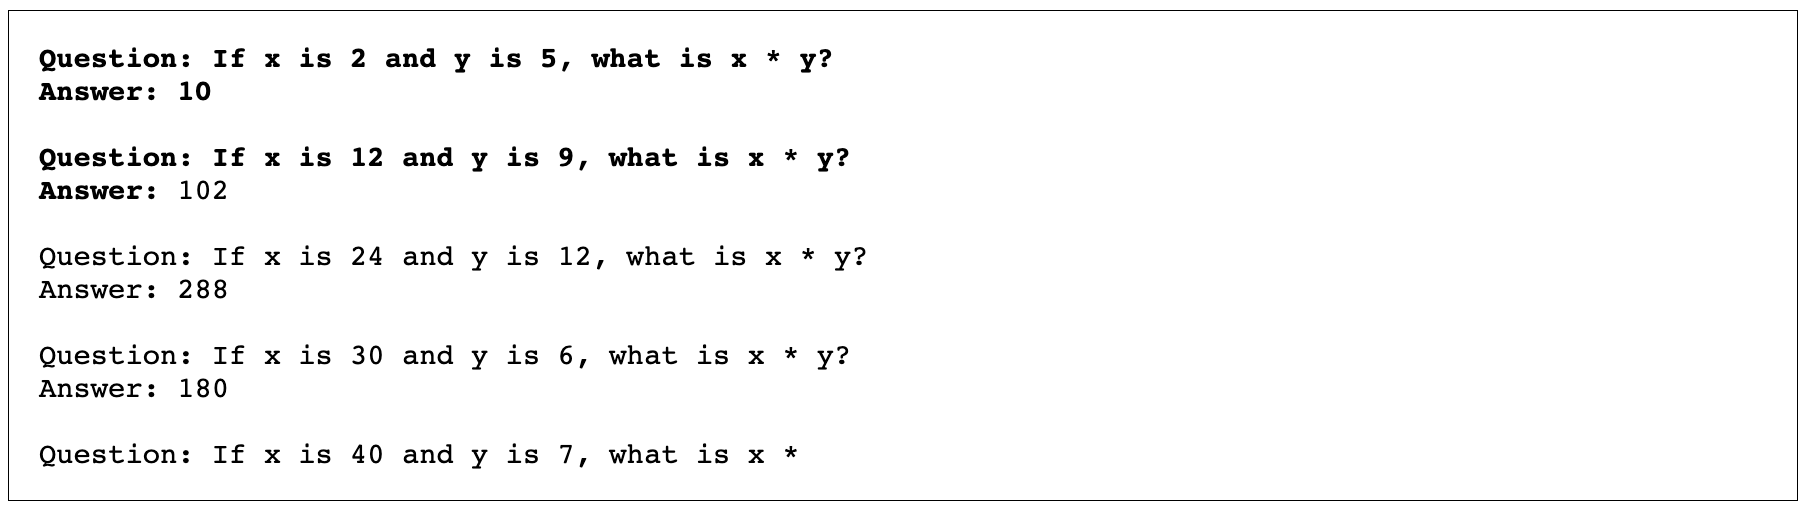
\includegraphics[width=1.0\textwidth]{samples/multiply_wrong.png}
    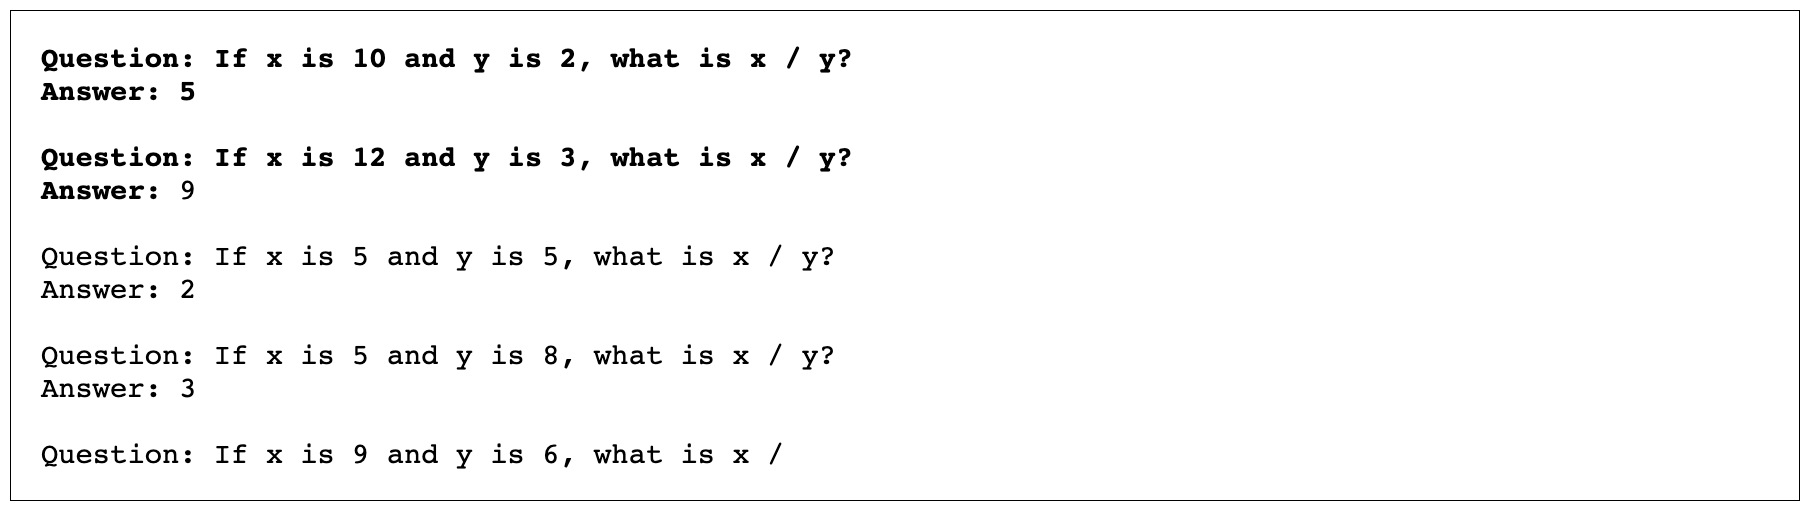
\includegraphics[width=1.0\textwidth]{samples/bad_division.png}
    \caption{{\bf Arithmetic.} We observe mistakes when extending from addition to other operations.}
    \label{fig:arithmetic}
\end{figure}

\begin{figure}[h]
    \centering
    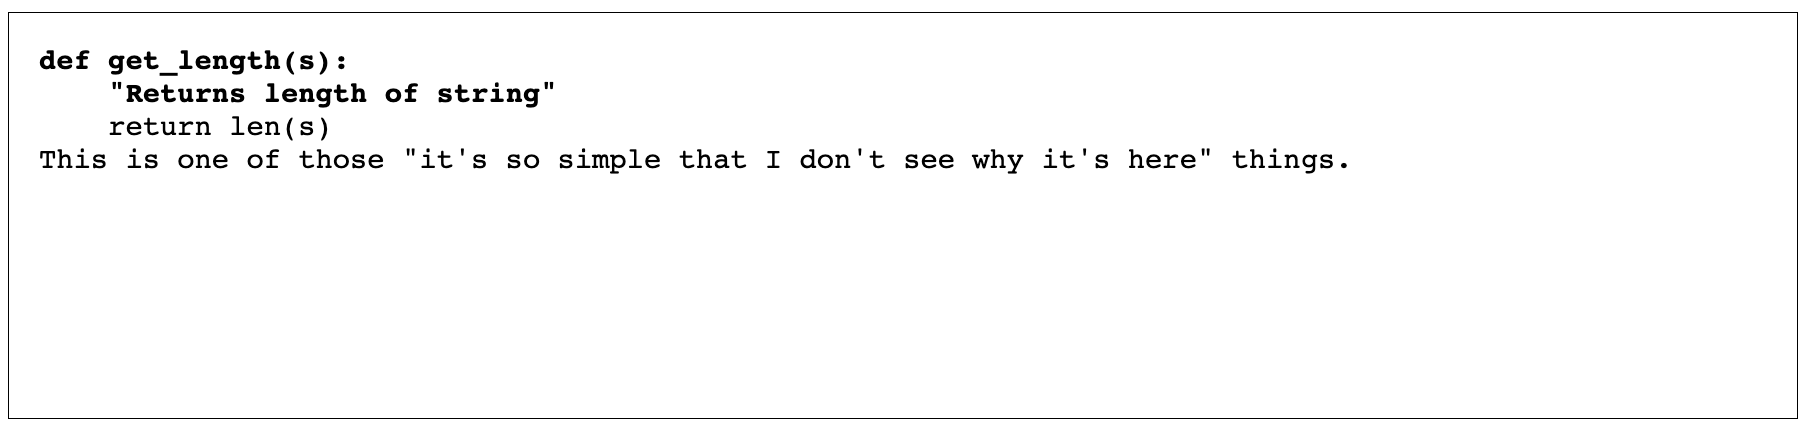
\includegraphics[width=1.0\textwidth]{samples/str_length.png}
    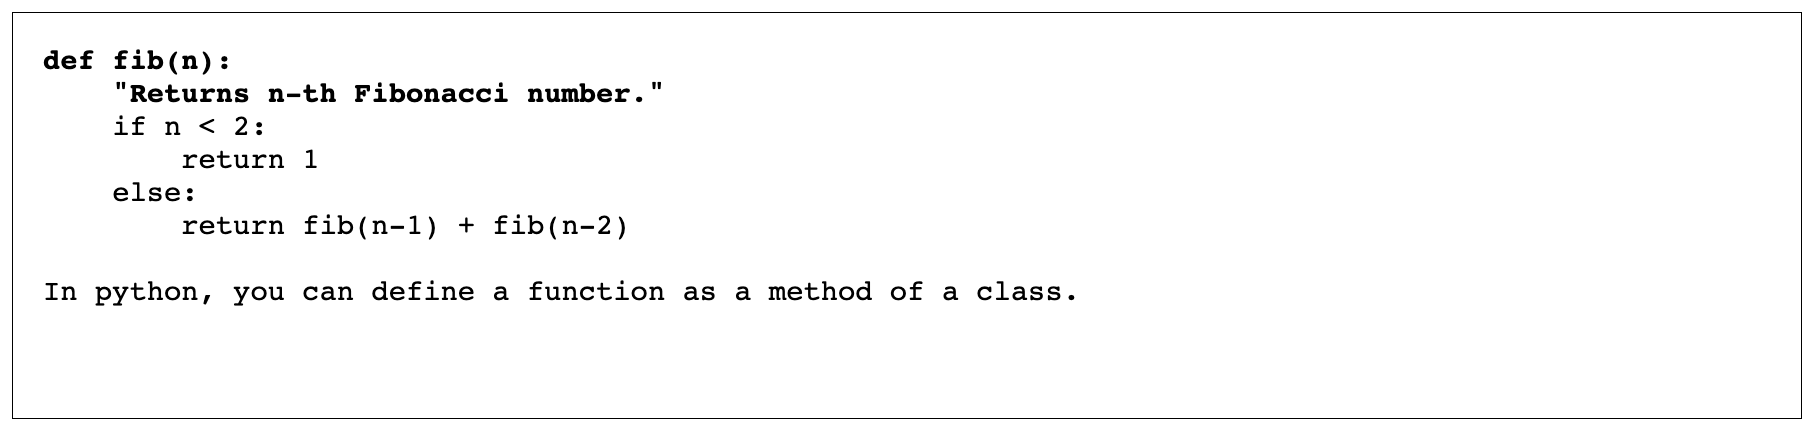
\includegraphics[width=1.0\textwidth]{samples/fib1.png}
    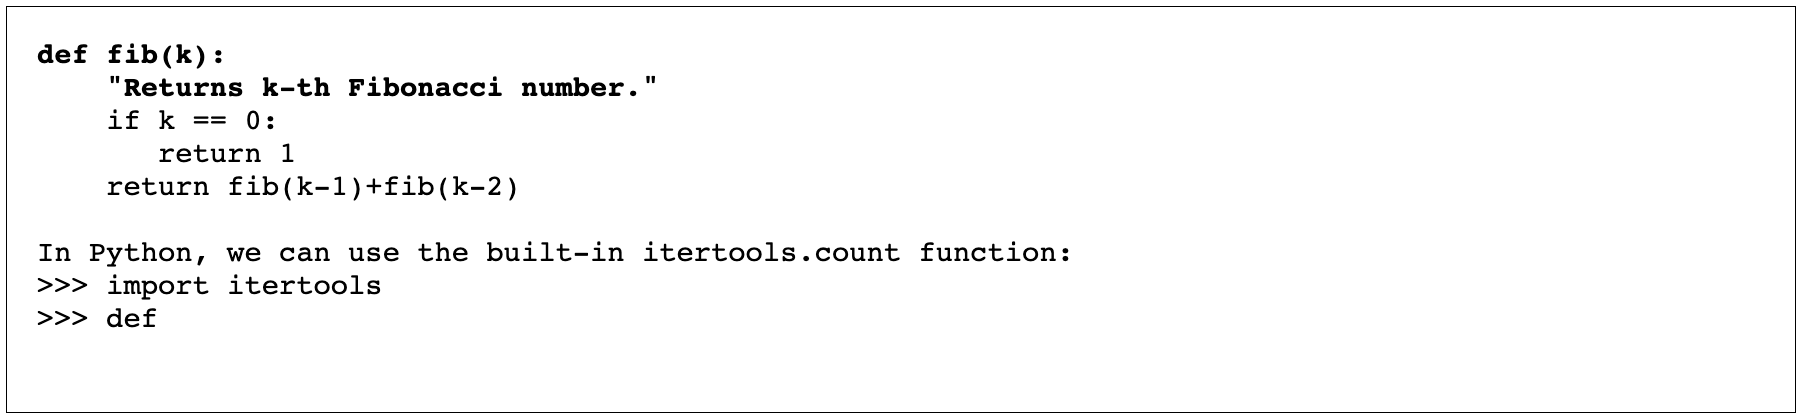
\includegraphics[width=1.0\textwidth]{samples/fib2.png}
    \caption{{\bf Python programming.} Simply switching out a variable name can alter the generated output.}
    \label{fig:python}
\end{figure}